% =====================================================================
%  VISAPP 2027 submission -- SCITEPRESS conference template
%
%  Format rules (from the VISAPP guidelines + template):
%   * Regular paper: 10,000--50,000 characters excluding spaces, INCLUDING
%     references, tables, figures and appendices. Accepted as Full Paper
%     (12 pages) or Short Paper (8 pages) in the proceedings.
%   * Double-blind: no author names, affiliations, acknowledgements or
%     self-identifying links (e.g. GitHub) in the submitted PDF.
%     Self-cite in the third person ("Smith et al. showed ..."), and keep
%     self-citations <= 20% of the references. Don't post a preprint while
%     the paper is under review.
%   * Abstract 70--200 words. At least one keyword, titlecased, comma
%     separated, ending with a period.
%   * Section titles in ALL CAPS (\uppercase), subsections titlecased.
%   * Table captions ABOVE the table, figure captions BELOW, every caption
%     ends with a period. Write "Figure"/"Table" in full in the text.
%   * Citations in APA (author, year) style: use \cite{} -- apalike does it.
%   * Do NOT edit article.cls, apalike.*, SCITEPRESS.sty.
%   * Add your own packages BEFORE \usepackage{SCITEPRESS}.
%
%  Compiler on Overleaf: pdfLaTeX (Menu -> Compiler).
% =====================================================================

\documentclass[a4paper,twoside]{article}

\usepackage{epsfig}
\usepackage{subcaption}
\usepackage{calc}
\usepackage{amssymb}
\usepackage{amstext}
\usepackage{amsmath}
\usepackage{amsthm}
\usepackage[hidelinks]{hyperref}
\usepackage{multicol}
\usepackage{pslatex}
\usepackage{apalike}
\usepackage{algorithm2e}
\usepackage[bottom]{footmisc}
% --- own packages (must come before SCITEPRESS.sty) -------------------
\usepackage{graphicx}
\usepackage{booktabs}
\usepackage{xcolor}
\usepackage{xspace}
\usepackage{SCITEPRESS}

% --- writing helpers ---------------------------------------------------

\newif\ifshowtodos \showtodostrue
\DeclareRobustCommand{\todo}[1]{\ifshowtodos{\color{red}\textbf{[TODO: #1]}}\fi}
\newif\ifblind \blindtrue


\newcommand{\catvton}{CatVTON\xspace}
\newcommand{\ootd}{OOTDiffusion\xspace}
\newcommand{\idm}{IDM-VTON\xspace}
\newcommand{\vitonhd}{VITON-HD\xspace}
\newcommand{\axis}[1]{\textsf{#1}}  

\begin{document}

% Title rules: titlecased, no formulas/special characters, subtitle after a colon.
\title{When Is the Garment Settled? \\ A Trajectory Analysis of Diffusion-Based Virtual Try-On}



\author{\authorname{Anonymous Submission}
\affiliation{}
\email{}
}


\keywords{Virtual Try-On, Diffusion Models, Denoising Trajectory, Interpretability.}

\abstract{Diffusion-based virtual try-on models produce realistic images of a person wearing a given garment. However, they are mostly evaluated on their final output. Little is known about how that output emerges during denoising. We decode the model's estimate of the clean image at every denoising step and score it on six axes: pose, structure, colour, texture, pattern and stability. We compare CatVTON, OOTDiffusion and IDM-VTON on 48 VITON-HD person-garment pairs, six in each of eight garment categories. All models use the same sampler and are scored over the same garment region at a common resolution. We also decompose every estimate into coarse, mid and fine spatial-frequency bands. All three models fix the pose and coarse structure of the garment within the first few steps and resolve fine detail last. They differ in timing: OOTDiffusion fills in the garment's texture and pattern from the first steps, whereas IDM-VTON and CatVTON only start to do so around step 5 and 10 respectively. Uniform garments reach their final structure within a few steps and then plateau, while repeating patterns keep changing much longer. These differences indicate where in the schedule each model could be improved or combined with another.

}

\onecolumn \maketitle \normalsize \setcounter{footnote}{0} \vfill

\section{\uppercase{Introduction}}
\label{sec:introduction}

Image-based virtual try-on, the task of rendering a given garment on a given person, has strong potential for online fashion retail, where customers cannot physically try on clothes. Latent diffusion models such as \catvton~\cite{chong2025catvton}, \ootd~\cite{xu2025ootdiffusion} and \idm~\cite{choi2024idmvton} now render these with striking realism. Though the technology has seen rapid development in recent years, it remains largely confined to research and has not yet seen mainstream adoption. Developing these models further is key to moving them from a "nice-to-have" experimental feature to a standard expectation across e-commerce. Allowing customers to virtually try on any item before purchase could reduce the number of returns, raise conversion rates and increase online shopping overall.  
\\ \\
To our knowledge, these models are mainly evaluated on their final image, using metrics such as FID~\cite{heusel2017fid}, KID~\cite{binkowski2018kid}, SSIM~\cite{wang2004ssim} or LPIPS~\cite{zhang2018lpips}, rather than on how that final image emerges over the denoising steps. Questions like whether the garment's colour is fixed before its print, whether the pose is fixed immediately or whether architecturally different models build the image in the same order remain largely unanswered. Insights into the dynamics of the diffusion process could be used to address weak points or to develop entirely new methods, for example by using multiple models throughout the denoising process and taking advantage of each one's main strengths. LPH-VTON~\cite{liu2026lphvton} uses this strategy by switching from a structure-biased to a texture-biased model through a Latent Process Handover.
\\ \\
We address this gap by studying how the try-on emerges during denoising rather than only evaluating the final image. At each denoising step, we decode the model's estimate $\hat{x}_0$ of the clean image and score it on six property-specific axes: pose, structure, colour, texture, pattern and stability. We compare \catvton, \ootd and \idm on 48 VITON-HD person-garment pairs, six in each of eight garment categories (check, dot, floral, graphic, lettering, solid, stripe and structural). All three models are run on the same 48 pairs with the same sampler. Each model generates at its own native resolution, but every estimate is resized to one common resolution and scored over the same garment region, so that the scores of the three models can be compared directly.
\\ \\
Our main contributions are as follows: 

\begin{itemize}
  \item A model-agnostic protocol to track garment properties along the
        denoising trajectory, with axes validated for specificity.
  \item A comparison of three diffusion VTON models over 48 garment-person pairs in eight garment categories.
  \item A frequency-band decomposition showing
that all three models generate the garment
from coarse to fine, but at a different pace.
  \item The finding that all three models fix pose and structure within the first few steps, though OOTDiffusion fills in the garment's detail earlier than CatVTON and IDM-VTON (from the first steps versus from around step 5 and 10 respectively), especially for repeating patterns such as stripes. 
\end{itemize}
\vspace{\baselineskip}
Section~\ref{sec:related} reviews related work, Section~\ref{sec:method} covers the trajectory analysis methodology and Section~\ref{sec:setup} the experimental setup. Following this, Section~\ref{sec:results} presents the results, which are further discussed in Section~\ref{sec:discussion}.

\section{\uppercase{Related Work}}
\label{sec:related}

\subsection{Image-Based Virtual Try-On}
Early try-on pipelines such as VITON~\cite{han2018viton} and VITON-HD~\cite{choi2021vitonhd} warp the garment onto the person and then blend it in with a generative adversarial network (GAN). More recent work replaces this approach with a latent diffusion model~\cite{rombach2022ldm} that is conditioned on the garment, for example LaDI-VTON~\cite{morelli2023ladivton} and StableVITON~\cite{kim2024stableviton}. The three models studied in this paper differ mostly in how they inject the garment into the denoising network. OOTDiffusion~\cite{xu2025ootdiffusion} encodes the garment with a distinct outfitting UNet and fuses its features into the self-attention layers of the denoising UNet. IDM-VTON~\cite{choi2024idmvton} leverages a pretrained diffusion model, SDXL~\cite{podell2024sdxl}, combined with a similar garment UNet (GarmentNet) for fine detail and an IP-Adapter~\cite{ye2023ipadapter} for high-level semantics. On the other hand, CatVTON~\cite{chong2025catvton} uses no extra encoder at all. The person and garment images are concatenated and processed by one inpainting UNet. Figure~\ref{fig:architectures} summarises these differences. All three works evaluate only the final image, with metrics such as FID, KID, SSIM and LPIPS. In contrast, we study how each model arrives at that image.

\begin{figure}[t]
  \centering
  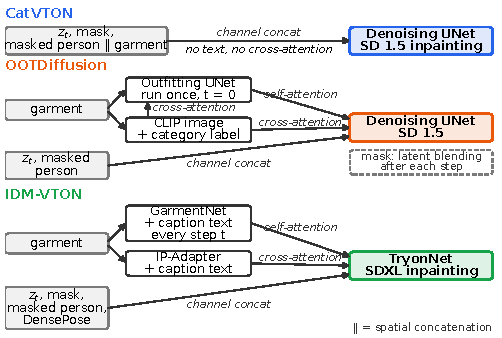
\includegraphics[width=\columnwidth]{figures/architectures.pdf}
  \caption{Inputs of the three models, with $z_t$ the noisy latent. \catvton places person and garment side by side ($\Vert$) in one inpainting UNet without text or cross-attention. \ootd and \idm encode the garment with a separate UNet whose features enter the self-attention layers. \ootd runs its outfitting UNet once before denoising, while \idm runs GarmentNet at every step. Through cross-attention, \ootd also receives the garment's CLIP image embedding with a category label, which is empty for the HD checkpoint used here. \idm receives an IP-Adapter embedding with a garment caption. \ootd uses the mask only to blend the latents after each step.}
  \label{fig:architectures}
\end{figure}


\subsection{Diffusion Models and Their Sampling Dynamics}
Diffusion models~\cite{ho2020ddpm} generate an image by gradually removing noise. With DDIM sampling~\cite{song2021ddim}, it is possible to sample them in fewer steps and to read out an estimate of the clean, final image at every step. Several works have observed that this process is coarse-to-fine, with high-noise steps responsible for coarse content and low-noise steps for detail~\cite{choi2022p2}. Since adding noise affects the high frequencies of natural images first~\cite{rissanen2023ihdm,dieleman2024spectral}, diffusion can also be seen as a frequency-ordered generation. High-level features, in turn, can be edited in the bottleneck of the UNet during the earlier steps~\cite{kwon2023hspace}. These studies concern unconditional or text-conditioned generation. In virtual try-on, however, the model is conditioned on a garment image which already contains all of the fine detail. Thus, it is not obvious that the same order holds. 

\subsection{Analysing Intermediate Predictions}
Usually, intermediate steps are used for editing rather than for analysis. Examples include SDEdit~\cite{meng2022sdedit}, which re-noises an image to an intermediate step before denoising it again and Prompt-to-Prompt~\cite{hertz2023p2p}, which injects attention maps during a chosen part of the trajectory. Both works rely on the intuition that different properties are decided at different steps. This method has also been applied in virtual try-on by LPH-VTON~\cite{liu2026lphvton} using latent hand-over from a structure-biased to a texture-biased model partway through denoising. To our knowledge, no prior work measures when the individual garment properties settle in different try-on models, which is what we address in this paper.


\section{\uppercase{Method}}
\label{sec:method}

\subsection{Capturing the Denoising Trajectory}
All three models are latent diffusion models that predict the noise $\epsilon_\theta(z_t, t, c)$ in a noisy latent $z_t$, given the conditioning $c$ (person, garment and pose inputs). From this prediction, the model's current estimate of the clean latent follows:

\begin{equation}
\hat{z}_0^{(t)} = \frac{z_t - \sqrt{1-\bar{\alpha}_t}\,\epsilon_\theta(z_t, t, c)}{\sqrt{\bar{\alpha}_t}}
\label{eq:x0}
\end{equation}
where $\bar{\alpha}_t$ is the cumulative noise schedule. We decode $\hat{z}_0^{(t)}$ with the model's own VAE at every step and call the result $\hat{x}_0^{(i)}$, with $i = 0, \dots, N-1$ the step index. The noise prediction used is the one after classifier-free guidance, like the one used in the sampler. For all three models, we verified at the first step of every run that Equation~\ref{eq:x0} reproduces the estimate that the scheduler computes internally.
\\ \\
To compare the models step by step, they must follow the same noise schedule. Therefore, all three models are sampled with DDIM~\cite{song2021ddim} using $\eta = 1$ and $N = 50$ steps, at the timesteps $t = 981, 961, \dots, 1$, i.e.\ every 20th of the 1,000 training timesteps. For CatVTON this is the default sampler and step count. OOTDiffusion and IDM-VTON use a different sampler by default (namely UniPC and DDPM respectively, both with 30 steps). Swapping the sampler does not change the network prediction for a given $z_t$ and $t$, since the noise schedule $\bar{\alpha}_t$ is a property of training, although the distribution of $z_t$ itself depends on the sampler. It does mean that the resulting final images vary slightly from the ones obtained with the original implementation. For CatVTON and OOTDiffusion, we re-implement the denoising loop step by step. Because IDM-VTON's pipeline contains considerable SDXL-specific conditioning, we leave its loop untouched and wrap the scheduler's step function, which receives $z_t$, $t$ and the guided noise prediction.

\subsection{Common Evaluation Frame}
The models do not work at the same resolution and use different inpainting masks. To make their scores comparable, we resize every frame to a resolution of $384 \times 512$ pixels, CatVTON's native resolution. All garment scores are computed over one shared region, namely the agnostic mask provided with VITON-HD, which covers both the garment and the arms. It therefore contains every pixel any of the models may repaint. Only pose is measured using the full frame.
\\ \\ 
All scores are reported on a $[0,1]$ scale. For the per-step curves, higher values indicate proximity to the final frame of the same run, $\hat{x}_0^{(N-1)}$, so every curve ends at 1. Consequently, the curves give an indication of how much of the final result is present at a given step, not how good that result is.

\subsection{Property Axes}
\label{sec:axes}
We define six axes, each targeting one property of virtual try-on output quality. 
\\ \\
\textbf{Pose.} OpenPose~\cite{cao2019openpose} detects the 18 COCO body keypoints on every frame, from which we compute the percentage of correct keypoints (PCK) with respect to the skeleton of the final frame. A keypoint is considered correct when it lies within a fraction $\tau$ of the torso length from its final position. To keep scores from changing in steps of $1/18$, we average over $\tau \in \{0.05, 0.1, 0.2\}$ for our final pose score, so that it changes gradually instead. We classify an undetected keypoint as incorrect. The OpenPose body model we used matches the one used by OOTDiffusion and IDM-VTON. It is also the model used to produce the VITON-HD keypoint annotations.
\\ \\
\textbf{Colour.} Both images are smoothed with a Gaussian of $\sigma = 4$ px and converted to CIELAB. Each garment pixel receives a score given by Equation~\ref{eq:s} that decreases continuously with its colour difference $\Delta E^*_{ab}$ to the final frame. Since a colour difference below $2.5$ is barely perceptible~\cite{mahy1994evaluation}, we truncate the score to 1 in this range. Above $\Delta E^*_{ab} = 20$, the difference is considered unacceptable and the score is set to 0. Between those thresholds, it decreases linearly in $\log \Delta E^*_{ab}$, so that every doubling of the difference reduces the score by a constant amount:
\begin{equation}
  s = \min\!\left(1, \max\!\left(0, \frac{\log(20 / \Delta E^*_{ab})}{\log 8}\right)\right).
  \label{eq:s}
\end{equation}
The mean of $s$ over all garment pixels produces the resulting colour axis value. The smoothing makes the axis compare the colour of regions rather than individual pixels, which would also react to noise and shifted edges.
\\ \\
\textbf{Structure.} The mean SSIM~\cite{wang2004ssim} over the garment pixels between the current frame and the final frame. Both are converted to greyscale and smoothed with a Gaussian of $\sigma = 2$ px to ensure noise and fine detail are not counted as structure.
\\ \\
\textbf{Texture.} The amount of fine detail compared to the final frame. We crop the garment region to its bounding box, fill the pixels outside the mask with the mean garment value and compute the power spectrum. The detail fraction $f$ is the share of spectral energy in the radial frequency band $0.1 < r \leq 0.3$, with $r = 1$ at the corner of the spectrum. The highest frequencies are left out so that residual noise does not count as detail. We compute the same fraction $f_{\text{ref}}$ for the final frame of the run and score each frame as $\min(f, f_{\text{ref}})/\max(f, f_{\text{ref}})$, so a frame with too little or too much detail scores low.
\\ \\
\textbf{Pattern.} Whether the generated garment's pattern matches that of the final frame, for example the period of a stripe or the repeat of a print. The score is calculated by resizing the garment crop to $128 \times 128$, computing the share of spectral power in 20 equal-width radial bins and comparing this profile $p$ to the profile $q$ of the final frame using $\exp(-\overline{|\log_{10} p - \log_{10} q|})$, where the bar denotes the mean over the 20 bins.
\\ \\
\textbf{Stability.} The mean SSIM over the garment pixels between a frame and the frame of the previous step. Unlike the other axes it does not use the final frame and measures how much the estimate is still changing. Therefore, it is undefined at step 0.
\\ \\
\textbf{Summaries.} We summarise each curve $s_i$ by one number. The trajectory AUC (Area Under the Curve) is the mean of the curve over all steps or in other words the normalised area under it. A high AUC means the frame is close to its final state for most of the trajectory. Curves with different shapes can have the same AUC, which is why we also report scores at fixed steps.

\subsection{Axis Validation}
\label{sec:validation}
Since an axis should only react to its own property and not to the others, we tested the sensitivity of each axis with controlled perturbations of the 144 final images. For the texture property, we applied a Gaussian blur to remove fine detail. By applying a constant shift in the $a^*b^*$ plane of CIELAB, it was possible to change only the colour of a frame and thus determine the colour scoring sensitivity. To evaluate the structure property, we applied a smooth random displacement field to move regions while retaining colour and detail. Finally, we also tested additive Gaussian noise, which no axis should react to. Pose and stability were not evaluated since pose relies on a keypoint detector and stability is a simple SSIM between consecutive frames.

\subsection{Frequency-Band Decomposition}
\label{sec:bands}
The structure and texture axes roughly follow coarse and fine content, but they cannot show which of the two a model resolves first. Each axis uses its own distance and its own mapping to $[0,1]$, so equal scores on two axes do not mean equal progress. The axes also start from different values at step 1. We therefore also decompose every frame $x$ in CIELAB into three spatial-frequency bands that sum back to the image,
\begin{equation}
x = \underbrace{G_8 * x}_{\text{coarse}} + \underbrace{(G_2 - G_8) * x}_{\text{mid}} + \underbrace{(x - G_2 * x)}_{\text{fine}},
\end{equation}
where $G_\sigma$ is a Gaussian blur of $\sigma$ pixels at the analysis resolution. Layout and large shading of the garment correspond to the coarse band. The mid band elements are sized roughly 2 to 8 pixels, such as stripes and dots. Edges and texture are taken into account by the fine band. Separately, we split each frame into luminance ($L^*$) and chroma ($a^*b^*$).
\\ \\
For each band $b$ at sampling step $i$, we compute the distance $d_b(i)$ to the same band of the final frame, weighted by a smoothed version of the garment mask. We define its progress as $p_b(i) = 1 - d_b(i)/d_b(1)$, clipped to $[0, 1]$. Each band is thus normalised by its own starting distance, so all bands go from 0 to 1 and can be compared directly. We start from step 1 rather than step 0 because \idm's estimate at step 0 ($t = 981$) is close to pure noise. At this step, Equation 1 divides by $\sqrt{\bar{\alpha}_t} \approx 0.08$, which amplifies any error in the guided noise prediction. From the band AUCs we define a coarse-to-fine index, $\text{AUC}_\text{coarse} - \text{AUC}_\text{fine}$, which is positive when coarse content is resolved before fine content. Likewise, the luminance-before-chroma index is $\text{AUC}_{L} - \text{AUC}_{ab}$.

\section{\uppercase{Experimental Setup}}
\label{sec:setup}

\subsection{Models}
We use the public VITON-HD checkpoints for all three models, given in Table~\ref{tab:models}. Every run uses the same seed (42), DDIM sampling with $\eta = 1$, 50 steps and the guidance scale recommended by the authors. Each model receives its inputs according to its official inference code; CatVTON its own agnostic mask, OOTDiffusion a mask derived from the human parsing and keypoints provided by VITON-HD and IDM-VTON the VITON-HD agnostic mask, a DensePose~\cite{guler2018densepose} map and a short garment caption.
\\ \\
For reference, Table~\ref{tab:models} also gives the FID and KID of the 48 final images of each model, computed against the 2,032 person images of the \vitonhd test split, with all images resized to $384 \times 512$. SSIM and LPIPS are not reported, since they need a ground-truth image of the person wearing the new garment, which does not exist in the unpaired setting. With only 48 images FID is biased upwards, so its values are only comparable within the table. The three models score almost the same (FID 84.2 to 84.7, overlapping KID ranges), so their final images are of similar quality.
\\ \\
\begin{table}[h]
\caption{Models and sampling settings. All models are sampled with DDIM, $\eta = 1$, 50 steps; CFG corresponds to the classifier-free guidance scale. FID and KID ($\times 10^3$, mean $\pm$ std over 1,000 subsets) of the 48 final images against the \vitonhd test images.}
\label{tab:models}
\centering
\small
\setlength{\tabcolsep}{3pt}
\resizebox{\columnwidth}{!}{%
\begin{tabular}{llcccc}
  \toprule
  Model & Backbone & Resolution & CFG & FID & KID \\
  \midrule
  CatVTON & SD 1.5 inpaint. & $384 \times 512$ & 2.5 & 84.7 & $4.0 \pm 2.1$ \\
  OOTDiffusion    & SD 1.5 + outfit.\ UNet & $768 \times 1024$ & 2.0 & 84.4 & $6.6 \pm 2.4$ \\
  IDM-VTON     & SDXL + GarmentNet & $768 \times 1024$ & 2.0 & 84.2 & $6.3 \pm 2.2$ \\
  \bottomrule
\end{tabular}}
\end{table}

\subsection{Data}
We evaluate on the \vitonhd~\cite{choi2021vitonhd} test split using the standard unpaired protocol, where each person is paired with a garment they are not wearing in the original image. To determine whether the denoising dynamics depend on the type of garment, they are grouped into eight categories that each highlight one visual property: \emph{solid} (uniform fabric, spread over different colours), \emph{lettering} (large text or logos), \emph{graphic} (one illustration), \emph{stripe}, \emph{floral}, \emph{dot}, \emph{check} (plaid and gingham) and \emph{structural} (solid fabric with buttons, pockets, zips or a peplum). Initially, we tried selecting the garments using the garment tags released with IDM-VTON, but we found that these were too noisy for this purpose; the ``dot'' tag, for example, occasionally returned plain tops. Therefore, we pre-filtered with the tags and chose the final garments by hand, six per category, for a total of 48 pairs. The image IDs of all pairs will be released with the code. We excluded lace, mesh, sequins and see-through fabrics, since they could have confounded the colour and texture measurements. Our usage of three models results in 144 trajectories and 7,200 decoded frames.

\subsection{Implementation Details}
All runs were performed on NVIDIA RTX 3090 Ti (24 GB) GPUs. Differences between models are tested with a paired Wilcoxon signed-rank test~\cite{wilcoxon1945} over the 48 pairs. The band indices are tested against zero with the same test. Differences between the eight garment categories are tested with a Kruskal–Wallis test~\cite{kruskal1952use}. No correction for multiple comparisons is applied, so results with $p \geq 0.01$ should be read as tendencies. The code will be released upon publication, together with the list of pairs.

\section{\uppercase{Results}}
\label{sec:results}

\subsection{Axis Validation}
% Figure~\ref{fig:axis_validation} shows the drop of each axis under the controlled perturbations. The colour axis drops by 0.34, 0.66 and 0.96 for colour shifts of $\Delta E^*_{ab} = 5$, 10 and 20. Under the same perturbation, the other three axes change by at most 0.02. Blur lowers the texture score by 0.64 at $\sigma = 2$\,px and by 0.81 at $\sigma = 4$\,px. At $\sigma = 2$\,px colour and structure change by less than 0.05. Beyond $\sigma = 4$\,px the texture score does not drop further. However, the stronger blur starts to affect colour (0.26) and structure (0.28) as well. Structure drops by 0.28, 0.41 and 0.49 for displacements of at most 16, 32 and 64 pixels, while the texture and pattern change by at most 0.14. The colour, however, does appear to change by 0.22, 0.35 and 0.48 with increasing warping. 

\noindent The validation in Figure~\ref{fig:axis_validation} shows two dependencies between axes. First, the colour axis reacts to displacement almost as strongly as structure does (0.22 to 0.48 against 0.28 to 0.49). Colour is compared at small, fixed pixel regions. Consequently, when a stripe moves, the colour at those positions changes. Structure, on the other hand, does not react to a colour shift. Second, the pattern axis reacts to blur (0.40 to 0.48), because removing fine detail also changes the shape of the spectrum. We therefore read texture and pattern together and interpret a low colour score as either a different colour or a displaced region. Noise with a standard deviation of 0.05 changes no axis by more than 0.05. At 0.2, colour and pattern drop by 0.23 and 0.24 respectively. This indicates that these two axes are less reliable on very noisy estimates.

\begin{figure}[t]
  \centering
  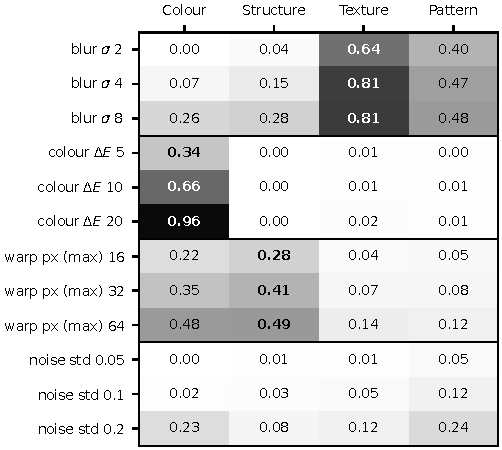
\includegraphics[width=\columnwidth]{figures/axis_specificity.pdf}
  \caption{Axis specificity: mean drop of each score under controlled perturbations of all 144 final images. Bold indicates which axis a perturbation targets.}
  \label{fig:axis_validation}
\end{figure}

\subsection{Order of Commitment Across Properties}
Figure~\ref{fig:curves_all} shows the mean curves of all six axes. In all three models, the pose and the coarse structure of the garment are fixed first. Texture, pattern and colour steadily improve throughout the sampling steps. The pose of the final image is present from step 1, meaning that the mean PCK with respect to the final skeleton is at least 0.95 from step 1 on in every model. The only exception is the estimate of IDM-VTON at step 0, which is close to pure noise and in which OpenPose often does not find a full skeleton (PCK 0.73). In every model, structure rises steeply in the first few steps, reaching 0.81 to 0.88 at step 10 and then increasing slowly until the last denoising step. 

\begin{figure*}[t]
  \centering
  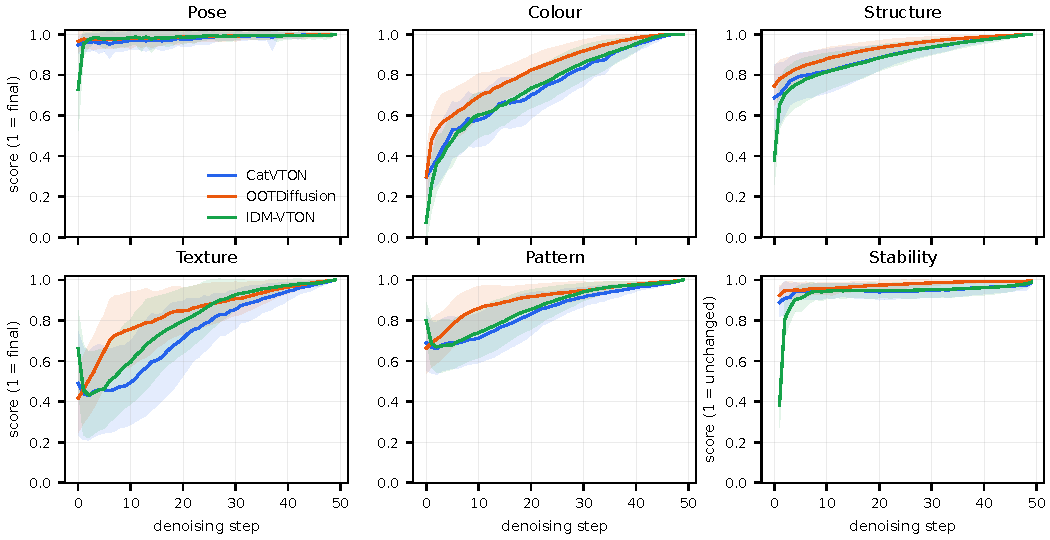
\includegraphics[width=\textwidth]{figures/curves_all.pdf}
  \caption{Per-step score of each axis, mean over the 48 pairs per model. The shaded band visualises $\pm 1$ standard deviation. Pose, colour, structure, texture and pattern are measured against the final frame of the same run, stability against the previous step.}
  \label{fig:curves_all}
\end{figure*}


\noindent Texture and pattern are resolved in a second phase. In CatVTON and IDM-VTON, the texture score first decreases from 0.49 to 0.44 in CatVTON and from 0.66 to 0.44 in IDM-VTON at step 3. These initial estimates contain a fair amount of noise. The estimate then becomes smooth. The texture score only rises again from around step 5 in IDM-VTON and step 10 in CatVTON. Colour rises at an almost constant rate until the last step, in CatVTON from 0.58 at step 10 to 0.83 at step 30 and in OOTDiffusion from 0.69 to 0.92. Since the band decomposition in Section~\ref{sec:res_bands} shows that chroma progresses as fast as luminance, however, this does not mean that the colour of the garment appears last. The colour axis requires most pixels to be within a small $\Delta E^*_{ab}$ of their final value and it also reacts to small displacements. Consequently, it keeps rising as long as regions are moving. The stability curves show that the estimate changes most in the first steps. After step 10, the step-to-step SSIM stays above 0.94 in every model, so the large changes happen early and are followed by many small corrections.
\\ \\
Figure~\ref{fig:x0_strip} shows an example with a striped garment. All three models settled the general layout and the shape of the top by step 5, but the stripes appear at different steps.
\\ 
\begin{figure}[t]
  \centering
  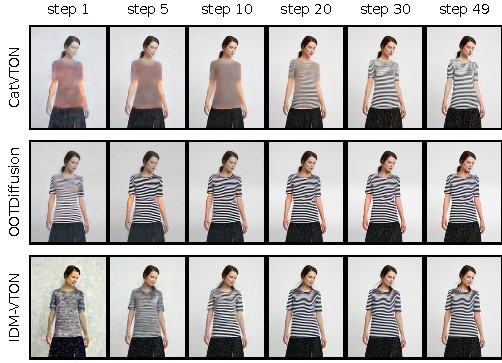
\includegraphics[width=\columnwidth]{figures/x0_strip.pdf}
  \caption{Decoded estimate $\hat{x}_0$ at six steps for one striped garment. \ootd shows the stripes from step 1, \idm from around step 5 and \catvton only from step 20.}
  \label{fig:x0_strip}
\end{figure}

\noindent Figures~\ref{fig:x0_strip_floral} and~\ref{fig:x0_strip_lettering} show two more examples. On the floral print, \ootd again shows the pattern from step 1, but \idm is now as late as \catvton: neither shows the flowers before step 20 and at step 5 \idm even shows horizontal stripes that are not in the garment. On the lettering, the large letters are readable by step 5 in all three models and only the small print below them appears later, between step 10 and 20.

\begin{figure}[t]
  \centering
  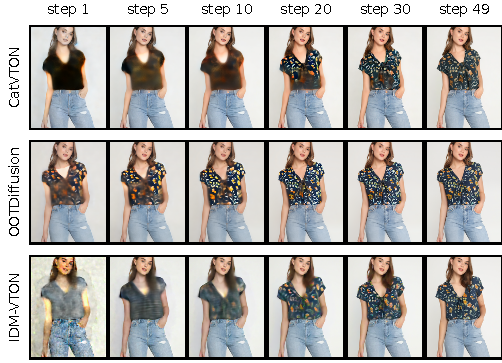
\includegraphics[width=\columnwidth]{figures/x0_strip_floral.pdf}
  \caption{Decoded estimate $\hat{x}_0$ for a floral print. \ootd shows the flowers from step 1, \catvton and \idm only from around step 20.}
  \label{fig:x0_strip_floral}
\end{figure}

\begin{figure}[t]
  \centering
  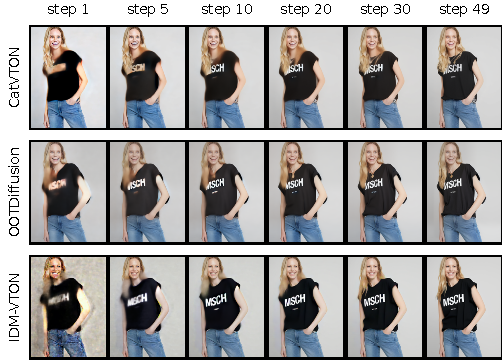
\includegraphics[width=\columnwidth]{figures/x0_strip_lettering.pdf}
  \caption{Decoded estimate $\hat{x}_0$ for a garment with large lettering. All three models show the lettering by step 5.}
  \label{fig:x0_strip_lettering}
\end{figure}

\subsection{Differences Between Models}
OOTDiffusion reaches its final state earlier than the other two models on every axis except pose, where all three are close to 1 from step 1. Its AUC is higher than that of both CatVTON and IDM-VTON for colour, structure, texture, pattern and stability ($p < 10^{-4}$ in every comparison, resulting from a paired Wilcoxon test over 48 pairs). The difference is most pronounced for texture and pattern. At step 10, the texture score of OOTDiffusion is 0.76, compared against 0.49 for CatVTON and 0.60 for IDM-VTON. Its pattern score is 0.86, against 0.71 and 0.74 respectively. CatVTON and IDM-VTON behave more similarly. Their colour AUC is nearly the same (0.749 and 0.751, $p = 0.92$). As suggested by LPH-VTON~\cite{liu2026lphvton}, CatVTON has a slightly higher structure AUC (0.894 against 0.883, $p = 0.01$), a weak indication that it is more structure-biased, while IDM-VTON has a higher texture AUC (0.801 against 0.743, $p < 10^{-3}$), making it more texture-biased. The lowest stability AUC was observed for IDM-VTON (0.935), primarily caused by the large change between step 0 and step 1 (SSIM 0.38). OOTDiffusion appears to be the most stable model. Its early commitment is not followed by extra compensation corrections later. None of these differences in timing shows up in the final images, whose FID and KID are almost the same for the three models (Table~\ref{tab:models}).

\subsection{Differences Between Garment Categories}
Figure~\ref{fig:summary_auc} gives the AUC per category, Figure~\ref{fig:curves_by_category} the mean curve per category for each model. Garments with large uniform areas (solid, lettering, graphic and structural) have a high structure AUC between 0.91 and 0.95 in every model, against 0.82 to 0.93 for the four repeating patterns (stripe, floral, dot and check). The Kruskal--Wallis test over the eight categories indicates that the difference between them is significant for structure in all three models ($p < 0.005$). This can already be observed at step 10. The uniform garments reach a structure score of 0.85 to 0.91 in CatVTON and IDM-VTON, the repeating patterns 0.73 to 0.79. In OOTDiffusion the gap is smaller, namely 0.89 to 0.93 against 0.84 to 0.88.
\\ \\
Texture exhibits the largest differences between both categories and models. In CatVTON, the texture score of stripes stays around 0.28 for the first ten steps and only rises steeply from about step 15. The floral and dot prints show a similar but smaller delay; 0.37 and 0.38 at step 10, compared to 0.73 for lettering. IDM-VTON shows the same delay for floral and dot prints; 0.36 and 0.38 at step 10, compared to 0.78 for lettering, but resolves stripes much earlier than CatVTON (0.66). In both models, the texture scores at step 10 differ by more than 0.4 between categories ($p < 0.005$) and the pattern scores by 0.24 to 0.28 ($p < 0.002$). In most categories, OOTDiffusion's texture curves rise in the first ten steps and lie close together. Floral prints are the exception: their texture score stays almost constant between step 10 and 30 and only then rises again.
\\ \\
The categories return similar results across models. The largest difference between models is observed for stripes. The texture AUC of CatVTON on stripes is 0.61, its lowest of all categories, against 0.83 and 0.91 for IDM-VTON and OOTDiffusion respectively. Its pattern AUC (0.79 against 0.88 and 0.93) and colour AUC (0.70 against 0.74 and 0.82) follow the same trend, which matches the example given in Figure~\ref{fig:x0_strip}. Colour differs less between categories: the AUC varies by 0.09 to 0.13 within a model. Only for CatVTON is this difference significant ($p = 0.02$). Lettering has the highest colour AUC in every model (0.81 to 0.87). It is worth noting that each category only contains six pairs, so these per-category results are means over a small number of garments.

\begin{figure*}[t]
  \centering
  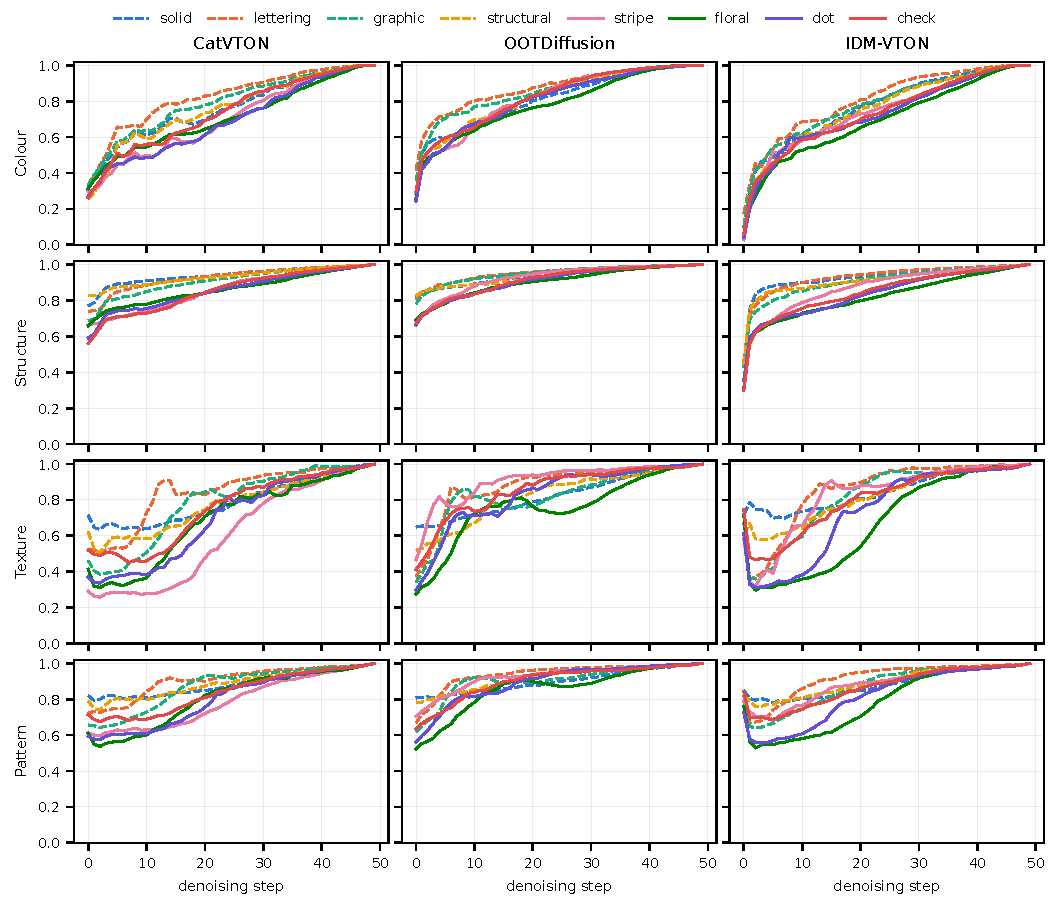
\includegraphics[width=\textwidth]{figures/curves_by_category.pdf}
  \caption{Mean per-step score of the four garment axes per category. Dashed lines are garments with large uniform areas, solid lines indicate repeating patterns.}
  \label{fig:curves_by_category}
\end{figure*}

\begin{figure*}[t]
  \centering
  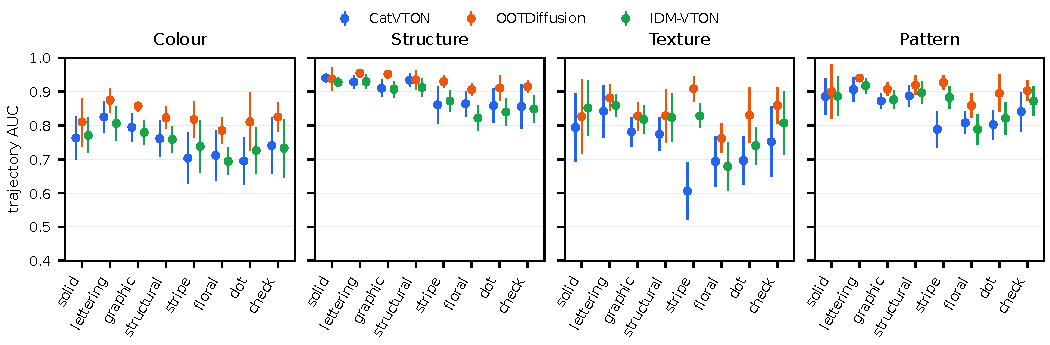
\includegraphics[width=\textwidth]{figures/summary_auc.pdf}
  \caption{Trajectory AUC of the four garment axes per category and model. Values are the mean over six pairs, with whiskers indicating $\pm 1$ standard deviation. Pose and stability are close to 1 in every category and are omitted.}
  \label{fig:summary_auc}
\end{figure*}

\subsection{Coarse-to-Fine Generation}
\label{sec:res_bands}
Figure~\ref{fig:band_progress} shows the progress of the three frequency bands. All three models generate the garment from coarse to fine. The coarse-to-fine index is positive in all 48 pairs for every model ($p < 10^{-14}$ against zero), with a median of $+0.46$ for CatVTON, $+0.43$ for IDM-VTON and $+0.30$ for OOTDiffusion. In CatVTON and IDM-VTON, the coarse band reaches half of its progress after approximately 10 steps, while the fine band changes little until the last third of the trajectory. OOTDiffusion is less coarse-to-fine than the other two models ($p < 10^{-8}$ against both), while CatVTON and IDM-VTON do not contrast significantly ($p = 0.07$). This is not because OOTDiffusion resolves the coarse band later given that its coarse AUC (0.64) is close to that of CatVTON (0.67). The difference lies in the fine band, which progresses almost linearly from the start in OOTDiffusion (fine AUC 0.34, against 0.22 for CatVTON and 0.29 for IDM-VTON).

\begin{figure*}[t]
  \centering
  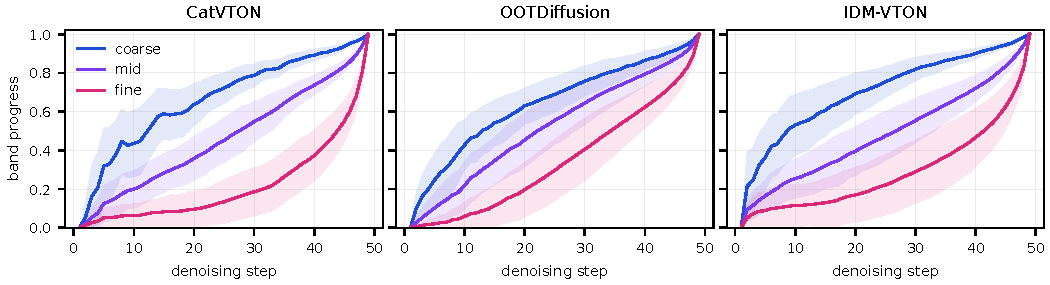
\includegraphics[width=\textwidth]{figures/band_progress.pdf}
  \caption{Progress of the coarse, mid and fine spatial-frequency bands towards the final frame, each normalised by its own distance at step 1 (mean over 48 pairs, $\pm 1$ standard deviation).}
  \label{fig:band_progress}
\end{figure*}
\vspace{\baselineskip}
\noindent In OOTDiffusion and IDM-VTON, luminance and chroma progress at the same rate; the median luminance-before-chroma indices ($+0.02$ and $+0.03$) do not differ significantly from zero. CatVTON resolves chroma before luminance in $79\%$ of the pairs (median index $-0.09$, $p < 10^{-4}$). Therefore, in CatVTON the colour of the garment is in place before its shading and fine structure.

\section{\uppercase{Discussion}}
\label{sec:discussion}

\textbf{Interpretation.} The overall observed order, with pose and coarse structure settling first while fine detail settles last, matches what is known about unconditional diffusion models~\cite{choi2022p2,rissanen2023ihdm}. Since in virtual try-on, the model uses a garment image that already contains all of the detail it needs to generate, this was not self-evident. Nonetheless, the models we evaluated still follow the natural frequency order imposed by the noise and the garment condition only has an effect on \emph{how early} the detail can be inpainted. This is where the models appear to vary. A possible explanation lies in how they inject the garment. OOTDiffusion, for example, processes the clean garment with a separate outfitting UNet and fuses those features into every self-attention layer of the denoising UNet. This way, detailed garment features are available from the first step, which fits its early rise in texture and pattern. On the other hand, CatVTON concatenates the garment to the person in the same input, causing the garment's detail to have to be propagated by the same network that is still resolving the noise. Finally, IDM-VTON also uses a separate garment UNet, but its timing is closer to CatVTON than to OOTDiffusion, therefore it appears that the garment encoder alone does not completely explain the difference. Additional possible factors that our study cannot separate include the base model (SDXL versus SD~1.5), the IP-Adapter, the different guidance scales and the different native resolutions. It is worth noting that although OOTDiffusion commits early, it also produces the most stable trajectories, so its early commitment does not come at the cost of more corrections later in the process.
\\ \\
\textbf{Implications.} Given that for all three models pose and structure settle within the first few steps, we conclude that the early steps fix the layout and the later steps primarily add the garment's appearance. This makes the second half of the trajectory, where texture, pattern and colour settle in \catvton and \idm, the place to intervene when print fidelity is the problem, for example with a stronger garment guidance in that part of the schedule. This result also supports a handover strategy like the one used in LPH-VTON~\cite{liu2026lphvton}. Given our measurements, the handover should happen around step 15 to 20 of 50 for CatVTON and IDM-VTON. Finally, the long, relatively flat tail of changes following the large modifications suggests that the number of sampling steps could be reduced, although the colour axis shows that the colours appear to be continuously refined until the end.
\\ \\
\textbf{Limitations.} The estimate $\hat{x}_0$ is merely an estimate of the final image, not the image itself. Accordingly, at high noise levels it is close to an average over many possible images. Therefore, a part of the coarse-to-fine behaviour is caused by the estimate rather than by the generation. This affects all models in the same way, however, thus the differences between models remain meaningful. Except for stability, our curves are measured against the final frame of the same run. Consequently, they show when a property reaches its final state, but not whether it was already decided at that point or merely becomes visible. Experiments that re-sample the noise from an intermediate step on would be needed to separate these two options. Furthermore, the axes are proxies. Colour is not independent of structure and pattern is not independent of texture. All results are on upper-body garments from a single dataset, with 48 pairs, one seed and one sampler per model. Two of the models were run with a sampler other than their default one. The standard scores in Table~\ref{tab:benchmark} are taken from the literature and were not measured on our runs. Finally, although all frames are scored at the same resolution, the models generate at their own native resolution ($384 \times 512$ for CatVTON, $768 \times 1024$ for the other two), which may affect how quickly fine detail appears.
\\ \\
\textbf{Future work.} To increase the confidence of these observations, natural next steps include evaluating more models and datasets, such as Dress Code~\cite{morelli2022dresscode} for lower-body garments and dresses. Additionally, restarting the generation from an intermediate step several times with fresh noise would show whether a property is already decided at that step, in which case it no longer varies across the restarts, or only becomes visible later.

\section{\uppercase{Conclusion}}
\label{sec:conclusion}

We studied the virtual try-on denoising dynamics instead of only using the final image for evaluation. By decoding the model's estimate of the clean image at every step and scoring it on six validated property axes, together with a frequency-band decomposition, we compared CatVTON, OOTDiffusion and IDM-VTON on 48 garment-person pairs in eight garment categories.
\\ \\
All three models generate the try-on in the same order: the pose and the coarse structure of the garment are fixed within the first few steps, after which the fine detail settles. The timing of when each axis settles, however, varies strongly between models. OOTDiffusion fills in the garment's detail much earlier than CatVTON and IDM-VTON. We found that the gap is largest for repeating patterns such as stripes, which CatVTON resolves particularly late. Looking at the trajectory rather than only the final image shows how each model uses its steps and could be used to determine in which part of the schedule a model could be improved or combined with another to obtain superior results.


\section*{\uppercase{Acknowledgements}}

\noindent\textbf{Use of AI tools.} The authors used Claude (Anthropic; Claude Opus 5.5, through Claude Code) as follows. All sections were written by the authors and only edited for language with Claude. Claude assisted with writing the code for running the three models, computing the scores and the band decomposition. It also assisted with the plotting code. The code for the FID/KID scores and the statistical tests was mostly generated by Claude and slightly edited by the authors. All experiments were run by the authors on their own infrastructure. Every image of a try-on or decoded estimate is an actual model output that was not altered. The authors decided the research questions and the experimental design. They checked the code and every reported number against the experiment outputs and take full responsibility for the content of this paper.

\bibliographystyle{apalike}
{\small
\bibliography{references}}




\end{document}
